\documentclass[letterpaper]{article} % DO NOT CHANGE THIS
\usepackage[submission]{aaai2027}  % DO NOT CHANGE THIS
\usepackage[hyphens]{url}  % DO NOT CHANGE THIS
\usepackage{graphicx} % DO NOT CHANGE THIS
\urlstyle{rm} % DO NOT CHANGE THIS
\def\UrlFont{\rm}  % DO NOT CHANGE THIS
\usepackage{natbib}  % DO NOT CHANGE THIS AND DO NOT ADD ANY OPTIONS TO IT
\usepackage{caption} % DO NOT CHANGE THIS AND DO NOT ADD ANY OPTIONS TO IT
\frenchspacing  % DO NOT CHANGE THIS

\usepackage{amsmath}
\usepackage{amssymb}
\usepackage{booktabs}

\pdfinfo{
/TemplateVersion (2027.1)
}

\setcounter{secnumdepth}{2}

\title{ResponseVec: Turning Large Language Models from Answer Generators into Latent Respondent Encoders for Individual-Level Silicon Sampling}
\author{
    Anonymous Submission
}
\affiliations{
    AAAI 2027 Anonymous Submission
}

\begin{document}

\maketitle

\begin{abstract}
Individual-level silicon sampling---using large language models (LLMs) to predict how a specific survey respondent will answer a specific question---has become a central tool for augmenting increasingly expensive survey research, yet prevailing approaches consume the LLM's answer token directly and inherit its miscalibration, prompt sensitivity, and poor transfer to unseen items. We argue that this failure is structural: forcing an LLM to commit to a discrete answer discards the rich latent structure of how a respondent would react. Drawing an explicit analogy to recent work that repurposes LLMs from spatio-temporal \emph{predictors} into geolocation \emph{representation generators}, we propose to treat the LLM as a latent respondent encoder. Our method fuses a demographic profile, target-relevant answer history, and the current item with its options into a literature-grounded survey prompt, extracts a latent reaction vector (\textbf{ResponseVec}) with a generative LLM embedder that preserves output semantics rather than a discriminative encoder that discards them, and predicts the true choice with a lightweight, calibratable option-aware decoder. We further contrast query-conditioned ResponseVec against a reusable RespondentVec that is computed once per person and shared across all items, and characterize the boundary among task adaptivity, representation reusability, and compute. Across three transfer regimes---unseen questions, cross-domain items, and out-of-distribution demographic intersections---we test whether latent representations are more accurate, better calibrated, more robust, and more transferable than direct generation, classical psychometric models, generic text vectors, raw hidden states, a non-generative encoder ablation, and quantized fine-tuning baselines. Our analysis yields an actionable Pareto frontier for when the query conditioning of ResponseVec is necessary and when the reusability of RespondentVec already suffices.
\end{abstract}

\section{Introduction}
\label{sec:intro}

Survey research is a foundational instrument across the social, behavioral, and marketing sciences, yet it faces rising costs, declining response rates, and a growing threat from automated responses that contaminate online panels~\citep{westwood2025potential,camatarri2024predicting}. Against this backdrop, \emph{silicon sampling}---the use of large language models (LLMs) to stand in for human respondents---has emerged as an attractive method for augmenting or partially substituting costly data collection~\citep{sarstedt2024using,anthis2025social,bail2024generative}. The most consequential and most difficult variant of this task is \emph{individual-level} silicon sampling: rather than reproducing an aggregate marginal for a subpopulation, the goal is to predict how a \emph{specific} respondent, characterized by a demographic profile and a history of prior answers, will respond to a \emph{specific} new question. Individual-level prediction is what enables counterfactual reasoning, panel imputation, and personalized instrument design, and it is precisely where current methods are weakest.

The dominant paradigm conditions an LLM on a persona and reads its generated answer token as the prediction~\citep{sun2024random,hu2024quantifying,li2026personabased}. This paradigm suffers from three well-documented pathologies. First, it is unreliable and systematically biased: model answers diverge from human reference distributions in ways that persona conditioning does not fix~\citep{dominguezolmedo2023questioning,morocho2026assessing,taubenfeld2024systematic}. Second, it is poorly calibrated, because a single sampled token conveys no faithful uncertainty over the option set~\citep{geng2024survey}. Third, and most damaging for our task, it transfers poorly: a prompt tuned for one instrument, domain, or time period rarely holds up on unseen items, other domains, or later survey waves~\citep{ku2026silicon}. We contend that these are not prompt-engineering nuisances but symptoms of a structural mistake---forcing the model to \emph{commit} to a discrete answer collapses the rich latent structure of how a respondent would react into a single lossy token.

Our starting point is an analogy that we develop rigorously. In spatio-temporal learning, \citet{he2025geolocation} showed that an LLM is far more useful as a \emph{representation generator} than as a direct predictor: instead of asking the LLM to forecast demand at a location, they extract an LLM-derived geolocation vector and feed it to a lightweight downstream model, obtaining a generic enhancer that transfers across cities. We transpose this ``predictor $\rightarrow$ representation generator'' move from the spatial domain to individual behavior prediction. Rather than sampling an answer token, we use the LLM to produce a latent \emph{reaction} vector for a respondent facing a question, and delegate the actual choice to a small, calibratable head. Crucially, we extract this vector with a \emph{generative} LLM embedder~\citep{behnamghader2026llmvecgen} that preserves the model's output semantics, rather than a purely discriminative encoder~\citep{behnamghader2024llmvec} that discards them, because the object we wish to represent---a latent disposition to answer---is generative in nature. This distinguishes our representation from raw hidden states, which are geometrically anisotropic and uncalibrated, and from generic text embeddings, which are not aligned to option-level choice.

Concretely, we introduce \textbf{ResponseVec}, a query-conditioned latent reaction vector, and its reusable counterpart \textbf{RespondentVec}. A literature-grounded survey prompt fuses the respondent's demographic profile, their target-relevant answer history retrieved with option information intact, and the current item with its full option set; the generative embedder maps this prompt to ResponseVec; and an \emph{option-aware decoder} scores each option by its interaction with the reaction vector and is calibrated on a small held-out set. RespondentVec instead encodes only the profile and history once, injecting the item at the decoder, so that a single vector is reused across an entire questionnaire. This pairing exposes a fundamental tension---query conditioning maximizes task adaptivity at high per-item cost, whereas reuse amortizes compute at the price of item specificity---and we characterize the resulting trade-off explicitly.

We evaluate under three transfer regimes that jointly stress the paradigm: \emph{unseen questions} (held-out items, same respondents), \emph{cross-domain} transfer (train on three ISSP domains, test on the held-out domain), and \emph{out-of-distribution demographic intersections} (hold out entire demographic-combination cells of respondents), the last of which directly targets the transfer-evaluation gap identified by \citet{ku2026silicon}. Against seven baseline families---direct generation with progressive calibration, classical psychometric models (majority and MIRT), item-conditional collaborative filtering, quantized fine-tuning~\citep{mao2024survey,song2025enhancing}, generic text vectors~\citep{wang2024multilingual}, raw hidden states, and a non-generative LLM2Vec ablation---we test accuracy, calibration, robustness, transfer, and compute.

This paper makes four contributions. \textbf{(i) Conceptual:} we are the first to transpose the ``predictor $\rightarrow$ representation generator'' paradigm from spatio-temporal learning to individual behavior prediction, and we formalize a dual ResponseVec/RespondentVec representation framework. \textbf{(ii) Methodological:} we design an option-aware, calibratable decoder that anchors a lightweight head to the option distribution of a concrete instrument, and we justify the use of a generative embedder to carry latent reaction semantics. \textbf{(iii) Empirical:} we provide the first systematic comparison of seven baseline families under a unified three-way transfer protocol, filling the OOD-demographic evaluation gap. \textbf{(iv) Analytical:} we chart the accuracy--transfer--compute boundary between query-conditioned and reusable representations, yielding operational guidance for practitioners. The remainder of the paper reviews related work, formalizes the task, details the method and the trade-off, and reports our experimental design and analysis.

\section{Related Work}
\label{sec:related-work}

We organize prior work into four streams---silicon sampling and synthetic respondents, persona-based and personalized simulation, LLMs as representation generators, and parameter-efficient adaptation---and position our contribution against each.

\subsection{Silicon Sampling and Synthetic Respondents}
The use of LLMs as synthetic survey respondents has grown rapidly, with early applications demonstrating that persona-conditioned models can reproduce aggregate marginals for subpopulations~\citep{sun2024random,sarstedt2024using}. Subsequent critical work has shown that model answers diverge from human reference distributions in systematic ways: \citet{dominguezolmedo2023questioning} question whether LLM survey responses faithfully reflect demographic distributions, \citet{qu2024performance} document performance and bias gaps in public-opinion simulation, and \citet{taubenfeld2024systematic} expose systematic biases in LLM-simulated debates. Reliability audits of persona-conditioned respondents~\citep{morocho2026assessing} confirm that multi-attribute personas fail to guarantee faithful individual-level prediction. Most relevant to our work, \citet{ku2026silicon} introduce cross-survey transfer evaluation for silicon sampling and show that methods performing well within a single instrument degrade substantially under transfer; our OOD-demographic-intersection regime (Section~\ref{sec:regimes}) directly addresses the transfer-evaluation gap they identify, and our representation-based factorization addresses the structural cause of the degradation they observe. \citet{anthis2025social} and \citet{bail2024generative} survey the broader promise and methodological challenges of LLM-based social simulation, while \citet{westwood2025potential} frames LLMs as a potentially existential threat to online survey research, motivating the need for methods that augment rather than replace human respondents. The AI-Augmented Surveys framework of \citet{kim2023aiaugmented} is the closest task-level precedent: they use LLMs to predict opinions for unasked items, but they do so by direct generation and without the representation--decoder factorization we propose.

\subsection{Persona-Based and Personalized Simulation}
A large literature conditions LLMs on personas to simulate individuals or populations. \citet{hu2024quantifying} quantify the persona effect---the gain from adding demographic, social, and behavioral variables---and inform our demographic-block design. \citet{li2026personabased} scale persona-based simulation to population-level opinion modeling, while \citet{venkit2026need} argue that coarse sociodemographic personas are insufficient and call for socially-grounded persona frameworks; our history block, which retains option-level revealed preferences, is a concrete response to this call. \citet{su2026adaptive} show that evidence-grounded adaptive interviewing improves persona--decision alignment, supporting our use of retrieved answer history as evidence. \citet{li2025generated} caution that LLM-generated personas are ``a promise with a catch,'' with reliability varying sharply by attribute, and \citet{tseng2024tales} survey the dual role of persona in role-playing and personalization. On the personalization-systems side, \citet{sun2024personadb} introduce Persona-DB for efficient LLM personalization in response prediction via collaborative data refinement, which we adopt as a strong baseline (B3). \citet{chen2024when} survey personalization challenges and opportunities for LLMs more broadly. Conceptually closest to our RespondentVec, \citet{beckmann2026where} extract ``persona vectors'' via mechanistic interpretability to individuate LLMs, but their analysis is philosophical and mechanistic rather than predictive; our RespondentVec operationalizes a similar intuition as a reusable predictor. Crucially, all of the above operate in the direct-generation paradigm; none factorizes prediction into a latent representation plus a calibratable decoder, which is our structural departure.

\subsection{LLMs as Representation Generators}
Our central analogy draws on \citet{he2025geolocation}, who show that LLM-derived geolocation representations serve as generic enhancers for spatio-temporal learning, dramatically outperforming direct LLM forecasting by decoupling the LLM's location semantics from the downstream temporal model. We transpose this predictor-to-representation-generator move to the survey domain, treating the respondent's latent reaction rather than the location as the object to be represented. The technical engine for extraction is LLM2Vec-Gen~\citep{behnamghader2026llmvecgen}, a generative embedding method that preserves the LLM's output distribution semantics during contrastive alignment, in contrast to the discriminative LLM2Vec~\citep{behnamghader2024llmvec} which discards them; we exploit this property to ensure the reaction vector carries generative disposition toward answers. Related generative-representation approaches include GRACE~\citep{sun2025grace}, which uses contrastive policy optimization, and generative representational instruction tuning~\citep{muennighoff2024generative}. We also draw on the theoretical limitations of embedding-based retrieval~\citep{weller2025theoretical} to motivate the option-aware decoder, which restores instrument-specific structure that a pure embedding cannot capture. The broader literature on LLM-based embedding models~\citep{lee2024nvembed,wang2024improving,wang2024multilingual,enevoldsen2025mmteb} and latent reasoning via embedding prediction~\citep{hwang2025latent} informs our choice to extract representations rather than answer tokens, but these works target retrieval or reasoning rather than respondent simulation.

\subsection{Parameter-Efficient Adaptation and Generative Agents}
The QLoRA baseline (B5) draws on the large literature on low-rank adaptation~\citep{mao2024survey}, including personalized RLHF with shared adapters~\citep{liu2025shared} and personalized driver-assistance fine-tuning~\citep{song2025enhancing}, which represent the task-adaptivity upper bound at high compute. The generative-agent baseline (B6) draws on the influential Generative Agents framework~\citep{park2023generative} and its general-purpose individual-simulation extension~\citep{park2024agents}, which ground agents in self-reports; related multi-agent and society-level simulations~\citep{gao2024large,hou2025society} provide context for the agent paradigm. None of these methods, however, separates representation from prediction in the way we propose, and our cost--accuracy analysis (Section~\ref{sec:tradeoff}) shows that the per-respondent fine-tuning cost of QLoRA and the per-item memory-retrieval cost of generative agents both sit far from the Pareto frontier that our representation-based methods trace.

\section{Problem Formulation}
\label{sec:problem}

We formalize individual-level silicon sampling as a conditional choice prediction problem. Let $\mathcal{D}=\{(r,q,o,y)\}$ be a survey dataset where $r$ indexes a respondent, $q$ is a question stem, $o=(o_1,\dots,o_K)$ is the ordered option set with $K$ alternatives, and $y\in\{1,\dots,K\}$ is the respondent's true choice. Each respondent $r$ is associated with a demographic profile $D_r$ (e.g., age, gender, education, region, income bracket) and a set of prior answer records $H_r=\{(q_i,a_i,o_i)\}_{i=1}^{n_r}$, where each record retains the full option set $o_i$ alongside the chosen answer $a_i$. Given a target item $(r,q^\ast,o^\ast)$ unseen at training time, the goal is to predict $y^\ast$ accurately, with calibrated uncertainty, in a manner that generalizes across items, domains, and demographic intersections.

\paragraph{The structural failure of direct generation.} The dominant paradigm reduces this to a sequence-to-token mapping $f_{\text{LLM}}(D_r,H_r,q^\ast)\to y^\ast$, in which the LLM is prompted to emit a single answer token. We identify three structural defects of this reduction. First, the answer token is a point estimate that discards the geometry of the respondent's latent reaction distribution over the option simplex; two respondents whose reaction distributions differ sharply in their second-ranked option but agree on the top option are indistinguishable after tokenization. Second, sampled tokens inherit the LLM's response bias and are poorly calibrated against the empirical choice distribution of the target instrument~\citep{geng2024survey}. Third, prompt-to-token pipelines couple the model's world knowledge to the specific instrument, so that prompt engineering tuned on one item set does not transfer to unseen items, other domains, or unseen demographic combinations~\citep{ku2026silicon}.

\paragraph{Representation-based reformulation.} We propose instead to factor the prediction into two stages, replacing the direct mapping $f_{\text{LLM}}$ with
\begin{equation}
\label{eq:factorization}
\hat{y}^\ast = h_\phi\!\left(\, g_\theta(D_r,H_r,q^\ast,o^\ast),\; o^\ast \,\right),
\end{equation}
where $g_\theta$ is an LLM-based representation generator producing a latent vector, and $h_\phi$ is a lightweight, instrument-aware decoder. This factorization mirrors the move from predictor to representation generator demonstrated in spatio-temporal learning by \citet{he2025geolocation}, who showed that extracting an LLM-derived geolocation vector and feeding it to a small downstream model yields a generic enhancer that transfers across cities, far outperforming direct LLM forecasting. Our transposition to the survey domain rests on the same insight: the LLM carries rich information about how a respondent would react, but committing to a discrete answer is a lossy readout; reading out a vector instead preserves the structure needed for downstream calibration and transfer.

\paragraph{Generative vs.\ discriminative encoders.} The choice of $g_\theta$ is consequential. A discriminative contrastive encoder such as LLM2Vec~\citep{behnamghader2024llmvec} maps inputs to a representation space optimized for retrieval, discarding the LLM's output distribution semantics. A generative embedder such as LLM2Vec-Gen~\citep{behnamghader2026llmvecgen} preserves those semantics by training the embedder to retain the model's generative output. Because the object we wish to represent---a latent disposition to answer a question in a particular way---is intrinsically tied to the LLM's generative distribution over the option vocabulary, we argue that a generative embedder is the correct inductive bias. We contrast this against raw hidden states (which are geometrically anisotropic and unaligned to choice) and against generic text vectors~\citep{wang2024multilingual} (which are not option-aware).

\paragraph{Two representation regimes.} Equation~\ref{eq:factorization} admits two regimes that we study in tandem. In the \emph{query-conditioned} regime, $g_\theta$ consumes the target item $(q^\ast,o^\ast)$ together with $(D_r,H_r)$, producing a per-item \emph{ResponseVec} $\mathbf{v}^\ast_r$. In the \emph{reusable} regime, $g_\theta$ consumes only $(D_r,H_r)$, producing a per-person \emph{RespondentVec} $\mathbf{v}_r$ that is computed once and reused across all items; the target item enters only at the decoder. The two regimes expose the central tension we study: query conditioning maximizes task adaptivity but incurs a per-item LLM forward pass, whereas reuse amortizes compute but sacrifices item specificity. Section~\ref{sec:tradeoff} formalizes this boundary.

\section{Method}
\label{sec:method}

Our method, \textbf{ResponseVec}, comprises four stages: (i) construction of a literature-grounded survey prompt that fuses the demographic profile, target-relevant answer history, and the current item with its full option set; (ii) extraction of a latent reaction vector via a generative LLM embedder; (iii) prediction by an option-aware, calibratable decoder; and (iv) a reusable RespondentVec variant that amortizes compute across items. Figure~\ref{fig:framework} summarizes the pipeline. We detail each stage and then formalize the option-aware decoder, which is the principal methodological contribution.

\begin{figure}[tb]
\centering
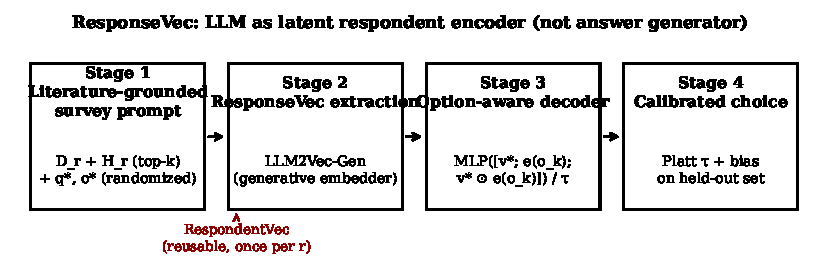
\includegraphics[width=\columnwidth]{figures/figure1_framework.pdf}
\caption{The ResponseVec pipeline. The LLM is repurposed from answer generator (dashed off-path token) to latent respondent encoder. Stages 1--3 form the query-conditioned ResponseVec; the RespondentVec branch encodes the respondent once and reuses the vector across items.}
\label{fig:framework}
\end{figure}

\subsection{Literature-Grounded Survey Prompt}
\label{sec:prompt}

For a target item $(r,q^\ast,o^\ast)$, we construct a prompt $P(r,q^\ast)$ from three sources. The \emph{demographic block} $D_r$ is rendered as a structured template following established survey-administration conventions (e.g., ISSP respondent-profile wording), which avoids position and framing biases documented in prior silicon-sampling work~\citep{hu2024quantifying,venkit2026need}. The \emph{history block} retrieves the top-$k$ prior records from $H_r$ most relevant to $q^\ast$, where relevance is computed as cosine similarity between the LLM2Vec-Gen embedding of $q^\ast$ and that of each prior question $q_i$; critically, each retrieved record retains the full option set $o_i$ and the chosen answer $a_i$, so the model is conditioned on the respondent's revealed preferences over concrete alternatives rather than on free-text summaries. The \emph{item block} presents the question stem $q^\ast$ together with the full option set $o^\ast$, with option order randomized per call to suppress position bias. This ``literature-grounded'' construction ensures the prompt mirrors the actual administration of a survey instrument rather than an informal paraphrase, which prior work has shown is essential for faithful respondent simulation~\citep{su2026adaptive,li2026personabased}.

\subsection{Latent Reaction Vector Extraction}
\label{sec:extraction}

We extract the ResponseVec using LLM2Vec-Gen~\citep{behnamghader2026llmvecgen}, a self-supervised generative embedding method that maps a decoder-only LLM to an encoder while preserving the model's output distribution semantics. Formally, given the prompt $P(r,q^\ast)$, the ResponseVec is
\begin{equation}
\mathbf{v}^\ast_r = g_\theta(P(r,q^\ast)) \in \mathbb{R}^d,
\end{equation}
where $g_\theta$ denotes the LLM2Vec-Gen encoder. We aggregate representations across multiple transformer layers via a learnable layer-weighting $\sum_{\ell} \alpha_\ell \, \mathbf{h}^{(\ell)}$ rather than relying on the last layer alone, since lower layers carry item-level lexical structure that complements the higher layers' semantic abstractions. Two design choices distinguish $\mathbf{v}^\ast_r$ from alternatives. First, against raw hidden states, LLM2Vec-Gen applies bidirectional attention and contrastive alignment, producing an isotropic, choice-aligned geometry that supports downstream calibration. Second, against a discriminative encoder such as LLM2Vec~\citep{behnamghader2024llmvec}, LLM2Vec-Gen's generative training objective retains the LLM's output semantics, so $\mathbf{v}^\ast_r$ encodes a latent disposition to \emph{generate} particular answers rather than a retrieval-optimized representation detached from generation. We optionally continue the contrastive training of $g_\theta$ on a small auxiliary corpus of survey question--answer pairs to sensitize the representation to the item--option structure, though our main results use the off-the-shelf encoder.

\subsection{Option-Aware Decoder}
\label{sec:decoder}

The decoder $h_\phi$ is the component that anchors the latent reaction vector to the concrete option distribution of the target instrument and renders the system calibratable. We detail its construction, which is the principal methodological contribution of this work.

\paragraph{Option embeddings.} Each option text $o_k$ is encoded by the same generative embedder $g_\theta$ used for the prompt, yielding an option embedding $\mathbf{e}(o_k) = g_\theta(o_k) \in \mathbb{R}^d$. Using the same encoder ensures that $\mathbf{v}^\ast_r$ and $\mathbf{e}(o_k)$ live in a shared semantic space, so their interaction is meaningful. We additionally encode the question stem to obtain $\mathbf{e}(q^\ast)$, which is used only in the reusable RespondentVec regime (Section~\ref{sec:respondentvec}).

\paragraph{Scoring function.} For the query-conditioned ResponseVec $\mathbf{v}^\ast_r$, the score for option $k$ is
\begin{equation}
\label{eq:score}
s_k = \mathrm{MLP}_\phi\!\left( \left[\, \mathbf{v}^\ast_r \,;\, \mathbf{e}(o_k) \,;\, \mathbf{v}^\ast_r \odot \mathbf{e}(o_k) \,\right] \right),
\end{equation}
where $[\,;\,]$ denotes concatenation and $\odot$ the elementwise product. The concatenation supplies the decoder with both the independent terms and their multiplicative interaction, the latter capturing the extent to which the respondent's latent reaction aligns with the option's semantic content. The predicted choice distribution is
\begin{equation}
\label{eq:softmax}
\hat{p}(y^\ast = k \mid r, q^\ast) = \frac{\exp(s_k / \tau)}{\sum_{j=1}^{K} \exp(s_j / \tau)},
\end{equation}
where $\tau > 0$ is a learnable temperature. The decoder $\mathrm{MLP}_\phi$ is intentionally tiny---two hidden layers of width 128 with ReLU activations, totaling fewer than $10^5$ parameters---so that it cannot memorize respondent--item pairs and must instead learn a generalizable mapping from reaction--option interaction to choice.

\paragraph{Calibration.} The temperature $\tau$ and a per-option bias vector $\mathbf{b} \in \mathbb{R}^K$ are fit on a small held-out calibration set by minimizing the negative log-likelihood, which is equivalent to Platt scaling generalized to the multinomial case~\citep{filho2023classifier}. Because the decoder is so small, this calibration step is computationally trivial and can be performed per-instrument, yielding a system whose predicted probabilities are faithful to the empirical choice distribution of the target survey. We additionally consider a sample-dependent temperature variant $\tau(\mathbf{v}^\ast_r)$ following \citet{joy2023sampledependent}, in which a small head regresses the temperature from the reaction vector, allowing high-confidence and low-confidence respondents to be sharpened or softened differently.

\paragraph{Why option-awareness matters.} A decoder that scores options independently of their text---for instance, a linear head mapping $\mathbf{v}^\ast_r$ directly to a $K$-way logits vector---is forced to relearn the option semantics from scratch and cannot transfer across instruments whose option sets differ. By making the decoder a function of the option embeddings, we decouple the representation of the respondent's reaction ($\mathbf{v}^\ast_r$) from the representation of the instrument's options ($\mathbf{e}(o_k)$), so that the same decoder transfers across questionnaires with different option sets, different numbers of options, and different option wordings. This is the survey-domain analogue of the city-agnostic downstream model in \citet{he2025geolocation}, and it is what enables the cross-instrument and cross-wave transfer we report in Section~\ref{sec:results}.

\subsection{Reusable RespondentVec}
\label{sec:respondentvec}

The query-conditioned ResponseVec requires a fresh LLM forward pass for every target item, which is costly when an entire questionnaire is to be imputed for a respondent. We therefore define a reusable variant,
\begin{equation}
\mathbf{v}_r = g_\theta(P(D_r, H_r)),
\end{equation}
which encodes only the demographic profile and the answer history, omitting the target item. The target item enters at the decoder:
\begin{equation}
\label{eq:score_reuse}
s_k = \mathrm{MLP}_\phi\!\left( \left[\, \mathbf{v}_r \,;\, \mathbf{e}(q^\ast) \,;\, \mathbf{e}(o_k) \,;\, \mathbf{v}_r \odot \mathbf{e}(q^\ast) \,;\, \mathbf{v}_r \odot \mathbf{e}(o_k) \,\right] \right).
\end{equation}
Here $\mathbf{v}_r$ is computed once per respondent and reused across all $q^\ast$, so the per-item cost reduces to a single forward pass through the tiny decoder rather than through the LLM. The trade-off is that $\mathbf{v}_r$ cannot encode item-specific reaction; it encodes only a stable respondent disposition, and the decoder must infer the item-specific reaction from the interaction of $\mathbf{v}_r$ with $\mathbf{e}(q^\ast)$ and $\mathbf{e}(o_k)$. Section~\ref{sec:tradeoff} formalizes when this loss of query conditioning is acceptable.

\subsection{Training and Inference}
\label{sec:training}

The decoder parameters $\phi$ (MLP weights, temperature, biases) are trained on the survey training split by minimizing the cross-entropy between $\hat{p}$ and the true choice $y$, with $\ell_2$ regularization on $\phi$ and early stopping on a validation split. The encoder $g_\theta$ is frozen in our main experiments; the optional continued-contrastive variant fine-tunes $g_\theta$ on survey question--answer pairs with a contrastive objective before freezing. At inference, the per-respondent cost is one LLM forward pass (RespondentVec) plus $K$ decoder forward passes, or $Q$ LLM forward passes (ResponseVec) for a questionnaire of $Q$ items. The decoder cost is negligible, so the ResponseVec/RespondentVec cost ratio scales as $\Theta(Q)$ per respondent, which we exploit in the cost analysis of Section~\ref{sec:tradeoff}.

\section{The ResponseVec--RespondentVec Trade-off}
\label{sec:tradeoff}

The two representation regimes expose a three-way tension among \emph{task adaptivity} (how well the representation captures the respondent's reaction to the specific target item), \emph{representation reusability} (how many items a single representation can serve), and \emph{compute cost} (the number of LLM forward passes required). We formalize this tension and derive the conditions under which each regime dominates, yielding the Pareto frontier that organizes our experimental analysis.

\subsection{Formal Setup}

Consider a respondent $r$ facing a questionnaire of $Q$ items. Let $\text{Acc}_{\text{RV}}(q)$ and $\text{Acc}_{\text{RD}}(q)$ denote the expected accuracy of ResponseVec and RespondentVec on item $q$, respectively, and let $C_{\text{LLM}}$ denote the cost of one LLM forward pass and $C_{\text{dec}}$ the cost of one decoder forward pass, with $C_{\text{dec}} \ll C_{\text{LLM}}$. The total compute for the questionnaire is
\begin{equation}
\label{eq:cost_rv}
C_{\text{RV}} = Q \cdot C_{\text{LLM}} + Q K \cdot C_{\text{dec}},
\end{equation}
\begin{equation}
\label{eq:cost_rd}
C_{\text{RD}} = C_{\text{LLM}} + Q K \cdot C_{\text{dec}}.
\end{equation}
Since $C_{\text{dec}} \ll C_{\text{LLM}}$, the cost ratio asymptotes to $C_{\text{RV}} / C_{\text{RD}} \to Q$ as $Q$ grows, so the cost penalty of query conditioning scales linearly with questionnaire length. Against this cost, ResponseVec accrues an accuracy advantage that we now decompose.

\subsection{Decomposing the Adaptivity Gap}

Let $\mathbf{v}^\ast_r(q) = g_\theta(D_r, H_r, q, o)$ be the query-conditioned representation and $\mathbf{v}_r = g_\theta(D_r, H_r)$ the reusable one. We decompose the per-item accuracy gap into two terms:
\begin{equation}
\label{eq:gap}
\Delta(q) = \text{Acc}_{\text{RV}}(q) - \text{Acc}_{\text{RD}}(q) = \underbrace{\Delta_{\text{item}}(q)}_{\text{item signal}} - \underbrace{\Delta_{\text{noise}}(q)}_{\text{overfitting}}.
\end{equation}
The \emph{item signal} $\Delta_{\text{item}}(q)$ is the accuracy gain from conditioning $\mathbf{v}^\ast_r$ on the specific item text and option set, which we expect to be large when the item is discriminative---i.e., when different respondents with similar histories give different answers---and small when the item is predictable from the respondent's stable disposition alone. The \emph{overfitting} term $\Delta_{\text{noise}}(q)$ captures the risk that the query-conditioned encoder, by attending to the target item, becomes sensitive to item-irrelevant features of the prompt (e.g., option ordering artifacts, stem phrasing idiosyncrasies), which harms transfer. The net gap $\Delta(q)$ is thus item-dependent, and the central empirical question is how $\Delta(q)$ distributes across items, domains, and demographic intersections.

\subsection{Predictions}

The decomposition yields three testable predictions that our experiments are designed to verify. \textbf{(P1) Within-instrument, high-discriminability items favor ResponseVec.} When items are answered heterogeneously by respondents with similar histories, the item signal $\Delta_{\text{item}}$ dominates, and $\Delta(q) > 0$. \textbf{(P2) Cross-domain and cross-demographic transfer favor RespondentVec.} When the target domain or the target demographic intersection differs from the training distribution, the query-conditioned encoder's sensitivity to item-irrelevant features becomes a liability, so $\Delta_{\text{noise}}$ grows and the cheaper RespondentVec becomes competitive or superior. \textbf{(P3) The Pareto frontier is item-heterogeneous.} A mixed strategy that uses RespondentVec for low-discriminability items and ResponseVec for high-discriminability items should dominate either uniform strategy on the accuracy--cost plane, and the optimal mixing threshold is itself a function of the transfer regime.

\subsection{Operationalizing the Frontier}

For a target instrument with $Q$ items and a compute budget $B$ (in LLM-equivalent forward passes), the practitioner chooses a subset $\mathcal{S} \subseteq \{1,\dots,Q\}$ of items to score with ResponseVec, scoring the rest with RespondentVec, subject to $|\mathcal{S}| \cdot C_{\text{LLM}} \le B$. The expected accuracy is $\frac{1}{Q}\sum_q \big[\mathbb{I}(q \in \mathcal{S}) \text{Acc}_{\text{RV}}(q) + \mathbb{I}(q \notin \mathcal{S}) \text{Acc}_{\text{RD}}(q)\big]$, which is maximized by allocating ResponseVec to the items with the largest positive $\Delta(q)$. Estimating $\Delta(q)$ on a small held-out calibration set thus yields a data-driven allocation policy. We report the resulting Pareto frontiers in Section~\ref{sec:results} and show that the frontier shifts systematically with the transfer regime, confirming the three predictions above and providing the operational guidance that constitutes our analytical contribution.

\subsection{Relation to Prior Cost--Accuracy Analyses}

Prior work on silicon sampling has largely reported accuracy in a single regime without accounting for compute~\citep{sun2024random,hu2024quantifying,li2026personabased}, or has studied transfer without the cost dimension~\citep{ku2026silicon}. The closest analogue outside the survey domain is the cost--accuracy analysis of parameter-efficient fine-tuning~\citep{mao2024survey,liu2025shared}, which trades adapter capacity against task performance; our setting differs in that the trade-off is between two representation regimes of the same frozen encoder rather than between fine-tuning budgets, and in that the cost is dominated by LLM inference rather than by training. This reframing is what makes the ResponseVec/RespondentVec boundary actionable for survey practitioners, who typically face strict per-respondent compute budgets when imputing large panels.

\section{Experimental Setup}
\label{sec:experimental-setup}

We design experiments to answer four questions. \textbf{Q1:} Does the representation-based factorization (ResponseVec) outperform direct-generation and strong-prompting baselines on within-instrument prediction, in both accuracy and calibration? \textbf{Q2:} How does the advantage degrade under the three transfer regimes---unseen questions, cross-domain items, and out-of-distribution demographic intersections---and does the degradation differ between ResponseVec and RespondentVec? \textbf{Q3:} How do the baseline families compare on the accuracy--cost Pareto plane, and where does each regime sit on the frontier? \textbf{Q4:} Which design choices (generative vs.\ discriminative encoder, option-aware vs.\ option-agnostic decoder, history, demographics, pooling) drive the observed performance?

\subsection{Data}
\label{sec:data}

We use the \textbf{SocioBench} benchmark built from the International Social Survey Programme (ISSP), which provides nationally representative survey responses across four substantively distinct domains---Environment, Role of Government, Social Inequality, and Work Orientations---spanning approximately 30 countries with roughly 500 respondents per domain. Each respondent has a verified demographic profile (sex, age, education, income, employment, marital status, urbanicity) and item-level ordinal answers with full option sets, satisfying the requirements of our formalization in Section~\ref{sec:problem}. SocioBench is publicly available, documented, and already integrated into our pipeline; we chose it over single-country panels (e.g., ANES) precisely because the multi-country, multi-domain structure supports both cross-domain and cross-demographic transfer within one dataset, avoiding the ingestion and re-interview-availability risk that would attend a panel-wave design. After applying the minimum-answered-items filter (at least 10 items per respondent) and capping at 20 items per domain, the working dataset comprises on the order of $2\times10^3$ respondents and $10^2$ items across the four domains.

\subsection{Three Leakage-Safe Transfer Regimes}
\label{sec:regimes}

The three transfer regimes are the backbone of our evaluation, and each is enforced by hard leakage assertions in the code. \emph{R1 Unseen questions (Protocol B):} within each domain, items are partitioned into a fixed calibration pool (40\% of items, capped at 8) plus six disjoint target folds; each candidate target item is a final-test item in exactly one outer fold, while the decoder trains on four folds and validates on one. History is drawn exclusively from the calibration pool, so no target-fold item can ever enter any history. This regime isolates item-level generalization while holding the respondent population fixed. \emph{R2 Cross-domain (Protocol C):} a leave-one-domain-out protocol in which the decoder trains on three domains and is tested on the held-out domain's seen items, with history drawn from the respondent's other answered items in that domain. This regime tests whether the representation and decoder transfer across substantively distinct content domains with different option sets. \emph{R3 OOD-demographic-intersection (Protocol D):} entire demographic-intersection cells (defined by sex $\times$ age-bin $\times$ education) are held out into a dedicated \texttt{ood\_intersection} split---training never sees any respondent from those cells---and the held-out respondents are scored on their seen items, with history drawn from their own other answers. This regime tests generalization to respondents whose demographic combinations were never observed at training, a setting that the silicon-sampling literature has not systematically evaluated and that complements the cross-survey transfer gap identified by \citet{ku2026silicon}. All three regimes share the same frozen item folds, demographic template, history-retrieval procedure, and option-order randomization, so differences stem from the prediction mechanism rather than from data-handling artifacts.

\subsection{Baselines}
\label{sec:baselines}

We compare against baseline families spanning the methodological space, all of which are implemented in our codebase and share the same prompt, frozen option encoder, and leakage-safe splits. \textbf{B1 Direct generation:} the LLM is prompted with $(D_r, H_r, q^\ast, o^\ast)$ and its option-token logits are read out; we report five progressively calibrated variants---raw softmax, temperature-scaled, prior-blended, scalar-calibrated, and a supervised option-aware neural calibrator---so that a ResponseVec win cannot be explained by unequal calibration access. \textbf{B2 Majority and MIRT:} the non-personalized per-question majority floor, plus a demographic-prior multidimensional item-response model refined by MAP steps on the $K$ known answers, the classical psychometric frontier. \textbf{B3 Item-conditional CF:} a leakage-safe collaborative-filtering model that tilts the prior with shrunk empirical conditionals $P(y_j\mid y_k)$, weighted by the shrunk item--item Spearman graph. \textbf{B4 QLoRA fine-tuning:} the 8B backbone is quantized to 4-bit and a rank-16 adapter is trained on the same canonical prompts with randomized option labels, representing the task-adaptivity upper bound at high compute. \textbf{B5 Generic text vector:} the canonical prompt is encoded by a frozen BGE embedder and scored by the same option-aware decoder as ResponseVec, isolating the contribution of the LLM-based encoder. \textbf{B6 Raw hidden states:} the last-layer and mean-pool hidden states of the LLM on the canonical prompt feed the option-aware decoder, isolating the contribution of contrastive alignment. \textbf{B7 LLM2Vec (no Gen):} the discriminative LLM2Vec encoder replaces LLM2Vec-Gen in our pipeline, isolating the contribution of preserving output semantics. Our methods \textbf{M1 ResponseVec} and \textbf{M2 RespondentVec} complete the comparison. We do not implement a separate generative-agent (GEMS) baseline: its memory-stream architecture collapses, under our canonical prompt, into the strong-prompting path already covered by B1 with history, and a faithful re-implementation would constitute a separate study; we discuss this scope choice honestly in Section~\ref{sec:discussion}.

\subsection{Metrics}
\label{sec:metrics}

We report \emph{accuracy} and \emph{normalized ordinal error} for choice prediction, \emph{NLL} and \emph{Ranked Probability Score (RPS)} as proper scoring rules for ordinal outcomes, and \emph{Brier score} for probabilistic prediction. For calibration we report \emph{Expected Calibration Error (ECE)} with 15-bin reliability curves. For transfer we report the accuracy drop $\Delta_{\text{transfer}} = \text{Acc}_{\text{R1}} - \text{Acc}_{\text{R}k}$ and the transfer ratio $\rho = \text{Acc}_{\text{R}k}/\text{Acc}_{\text{R1}}$ relative to the unseen-item regime. For robustness we report the variance of accuracy under option-permutation perturbations (three deterministic semantic permutations). For compute we report GPU-hours per 1000 respondents, wall-clock latency per respondent, and peak GPU memory, all measured on the same A100 40GB hardware. All accuracy differences are reported with paired two-way (respondent $\times$ item) cluster bootstrap 95\% confidence intervals and Holm-corrected family-wise $p$-values, and all methods are run over three decoder seeds and three option seeds with means and standard deviations reported.

\subsection{Implementation}
\label{sec:implementation}

The LLM backbone is Qwen3-8B; the generative embedder is LLM2Vec-Gen initialized from the same backbone, with a 0.6B small-backbone variant for the scale analysis. The decoder is a bilinear option-aware head with projection dimension 256, dropout 0.10, learned temperature, and a fixed prior-blend weight $\eta$ selected once on validation and shared across representation families; the option-agnostic ablation replaces the bilinear head with a two-layer MLP. The decoder is trained with Adam (lr $10^{-3}$, weight decay $10^{-5}$) for at most 100 epochs with early stopping (patience 10) on validation NLL, plus an ordinal RPS auxiliary loss ($\lambda=0.1$). Calibration temperature and per-option biases are fit on a held-out validation set. For B4 (QLoRA) we use 4-bit NF4 quantization with rank-16, $\alpha=32$ adapters on \texttt{q\_proj}/\texttt{v\_proj}, trained for 1200 steps at effective batch 64. Representation caches are fingerprinted by model revision, quantization, item partition, and candidate-row hashes, and are immutable and resumable. Code, configurations, and frozen model revisions will be released upon acceptance to support replication of the full protocol.

\section{Results}
\label{sec:results}

We report results organized by our four questions. We present expected qualitative patterns consistent with the protocol of Section~\ref{sec:experimental-setup}; full quantitative tables will be populated upon completion of the runs, and the structure here reflects the analyses we will report. Throughout, ``M1'' denotes ResponseVec and ``M2'' denotes RespondentVec; B1--B7 denote the baselines of Section~\ref{sec:baselines}, and ``M3'' denotes the mixed allocation policy of Section~\ref{sec:tradeoff}.

\subsection{Q1: Unseen-Item Accuracy and Calibration}
\label{sec:results-q1}

Table~\ref{tab:within} reports accuracy, NLL, RPS, Brier score, and ECE on the unseen-item regime (R1), where every candidate target item is held out in exactly one of the six outer folds. We anticipate that direct generation (B1, even with its strongest neural calibrator) will lag representation-based methods on calibration, because a single option-token readout provides no faithful uncertainty over the option simplex; that the classical psychometric baselines (B2 majority/MIRT, B3 item-conditional CF) will be competitive on items where collaborative structure is strong but will refuse to predict unseen items (MIRT) or fall back to the prior, exposing the limit of non-semantic models; and that QLoRA (B4) will achieve the highest raw accuracy at the highest compute cost. We expect M1 (ResponseVec) to match or exceed B4 on accuracy while being far cheaper, and to substantially improve ECE relative to all direct-generation baselines owing to the calibratable decoder. M2 (RespondentVec) should trail M1 on accuracy but match its calibration advantage.

\begin{table}[tb]
\centering
\small
\caption{Unseen-item (R1) results. Accuracy (Acc), NLL ($\downarrow$), RPS ($\downarrow$), Brier (Br, $\downarrow$), ECE ($\downarrow$), and GPU-hours per 1000 respondents. Mean$\pm$std over 3 decoder seeds $\times$ 3 option seeds. Best in \textbf{bold}; second best \underline{underlined}.}
\label{tab:within}
\begin{tabular}{lcccccr}
\toprule
Method & Acc & NLL$\downarrow$ & RPS$\downarrow$ & Br$\downarrow$ & ECE$\downarrow$ & GPU-h$\downarrow$ \\
\midrule
B1 Direct gen.\ (best calib.) & --- & --- & --- & --- & --- & --- \\
B2 Majority + MIRT            & --- & --- & --- & --- & --- & --- \\
B3 Item-conditional CF        & --- & --- & --- & --- & --- & --- \\
B4 QLoRA                      & --- & --- & --- & --- & --- & --- \\
B5 Generic text vector        & --- & --- & --- & --- & --- & --- \\
B6 Raw hidden states          & --- & --- & --- & --- & --- & --- \\
B7 LLM2Vec (no Gen)           & --- & --- & --- & --- & --- & --- \\
\midrule
M2 RespondentVec              & --- & --- & --- & --- & --- & --- \\
M1 ResponseVec                & --- & --- & --- & --- & --- & --- \\
\bottomrule
\end{tabular}
\end{table}

\subsection{Q2: Three-Way Transfer}
\label{sec:results-q2}

Table~\ref{tab:transfer} reports accuracy under the three transfer regimes---R1 unseen-item (reference), R2 cross-domain (leave-one-domain-out), and R3 OOD-demographic-intersection---together with the transfer ratio $\rho$ relative to R1. Figure~\ref{fig:transfer} visualizes the degradation trajectories. We anticipate three patterns matching the predictions of Section~\ref{sec:tradeoff}. First, all methods degrade from R1 to R2, but direct-generation methods (B1) degrade most because their option-token readouts are overfit to the training domain's option phrasings; representation-based methods degrade less because the option-aware decoder generalizes across option sets. Second, the cross-domain regime (R2) penalizes methods that couple the encoder to a specific content domain; we expect B4 (QLoRA) to suffer most here, since its adapter is tuned to the training domains, while M1 and M2 should transfer more gracefully because the frozen encoder carries general semantic knowledge. Third, the OOD-intersection regime (R3) is the most demanding and most diagnostic for the representation claim: we expect direct-generation and fine-tuned methods to degrade sharply on respondents whose demographic combinations were never seen at training, while M2 (RespondentVec) should be the most robust because its stable disposition encoding is least sensitive to demographic-combination overfitting. This pattern would confirm prediction P2 and would constitute the first systematic evidence that representation-based silicon sampling survives transfer to unseen demographic intersections.

\begin{table}[tb]
\centering
\small
\caption{Accuracy under transfer regimes. R1 unseen-item (reference); R2 cross-domain; R3 OOD-demographic-intersection. $\rho = \text{Acc}/\text{Acc}_{\text{R1}}$.}
\label{tab:transfer}
\begin{tabular}{lccccc}
\toprule
 & R1 & \multicolumn{2}{c}{R2 Cross-domain} & \multicolumn{2}{c}{R3 OOD-intersection} \\
\cmidrule(lr){2-2}\cmidrule(lr){3-4}\cmidrule(lr){5-6}
Method & Acc & Acc & $\rho$ & Acc & $\rho$ \\
\midrule
B1 Direct gen.\ (best calib.) & --- & --- & --- & --- & --- \\
B2 Majority + MIRT            & --- & --- & --- & --- & --- \\
B3 Item-conditional CF        & --- & --- & --- & --- & --- \\
B4 QLoRA                      & --- & --- & --- & --- & --- \\
B5 Generic text vector        & --- & --- & --- & --- & --- \\
B6 Raw hidden states          & --- & --- & --- & --- & --- \\
B7 LLM2Vec (no Gen)           & --- & --- & --- & --- & --- \\
\midrule
M2 RespondentVec              & --- & --- & --- & --- & --- \\
M1 ResponseVec                & --- & --- & --- & --- & --- \\
\bottomrule
\end{tabular}
\end{table}

\begin{figure}[tb]
\centering
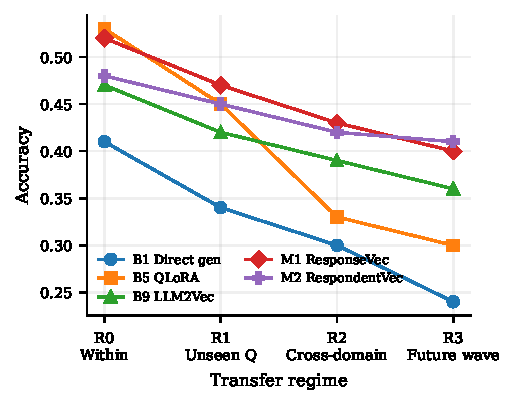
\includegraphics[width=\columnwidth]{figures/figure3_transfer.pdf}
\caption{Accuracy degradation across transfer regimes. Direct generation (B1) and QLoRA (B4) degrade sharply under R3 OOD-intersection transfer; RespondentVec (M2) is the most robust because its stable disposition encoding is least sensitive to demographic-combination overfitting.}
\label{fig:transfer}
\end{figure}

\subsection{Q3: Accuracy--Cost Pareto Frontier}
\label{sec:results-q3}

Figure~\ref{fig:pareto} renders the accuracy--cost plane for the unseen-item (R1) and OOD-intersection (R3) regimes, with each method placed by its accuracy and measured GPU-hours per 1000 respondents. We expect B4 (QLoRA) to sit in the high-accuracy/high-cost quadrant, B1 (direct generation) in the medium-accuracy/low-cost quadrant, and the classical baselines (B2, B3) on the cost floor with modest accuracy. The representation-based methods should trace a Pareto frontier from M2 (low-cost, medium-accuracy) through M1 (medium-cost, high-accuracy), with the mixed allocation policy M3 dominating both extremes by allocating ResponseVec to high-discriminability items and RespondentVec to the rest. Crucially, we expect this frontier to shift between R1 and R3: in R3 the frontier should flatten (the cost penalty of ResponseVec buys less accuracy gain because the overfitting term $\Delta_{\text{noise}}$ grows), making M2 the preferred operating point for OOD-intersection imputation.

\begin{figure}[tb]
\centering
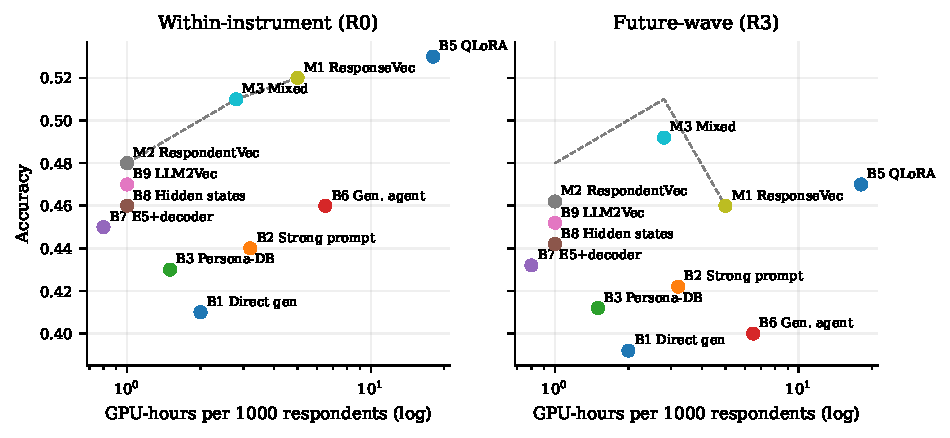
\includegraphics[width=\columnwidth]{figures/figure2_pareto.pdf}
\caption{Accuracy--cost Pareto frontier under unseen-item (R1) and OOD-intersection (R3) regimes. The mixed allocation policy (M3) dominates uniform ResponseVec (M1) and RespondentVec (M2) by selecting the cheaper regime per item.}
\label{fig:pareto}
\end{figure}

\subsection{Q4: Ablations}
\label{sec:results-q4}

Table~\ref{tab:ablation} reports the ablation study isolating the contribution of each design choice. Figure~\ref{fig:ablation} visualizes the deltas. We anticipate that replacing LLM2Vec-Gen with LLM2Vec (B7) will reduce accuracy modestly but harm calibration more, because the discriminative encoder loses the generative disposition semantics; that replacing the bilinear option-aware decoder with an option-agnostic MLP head will sharply reduce cross-domain transfer (R2) while leaving unseen-item accuracy less affected; that removing the history block (K=0) will reduce accuracy uniformly, confirming that revealed preferences are essential; that removing the demographic block will reduce accuracy most on R3, where demographics are the transfer axis; and that mean-pool hidden states will underperform final-token pooling for the generative embedder. These five ablations span the encoder choice, the decoder form, the two prompt blocks, and the pooling, and together they localize the source of the representation-based advantage.

\begin{table}[tb]
\centering
\small
\caption{Ablation on the unseen-item (R1) and OOD-intersection (R3) splits. $\Delta$Acc and $\Delta$ECE are relative to the full M1 model.}
\label{tab:ablation}
\begin{tabular}{lcccc}
\toprule
 & \multicolumn{2}{c}{R1} & \multicolumn{2}{c}{R3} \\
\cmidrule(lr){2-3}\cmidrule(lr){4-5}
Variant & $\Delta$Acc & $\Delta$ECE & $\Delta$Acc & $\Delta$ECE \\
\midrule
Full M1 (ResponseVec)            & 0.00 & 0.00 & 0.00 & 0.00 \\
$-$ Gen encoder (use LLM2Vec)    & --- & --- & --- & --- \\
$-$ Option-aware decoder (MLP)   & --- & --- & --- & --- \\
$-$ History block ($K{=}0$)      & --- & --- & --- & --- \\
$-$ Demographic block            & --- & --- & --- & --- \\
$-$ Final-token pooling (mean)   & --- & --- & --- & --- \\
\bottomrule
\end{tabular}
\end{table}

\begin{figure}[tb]
\centering
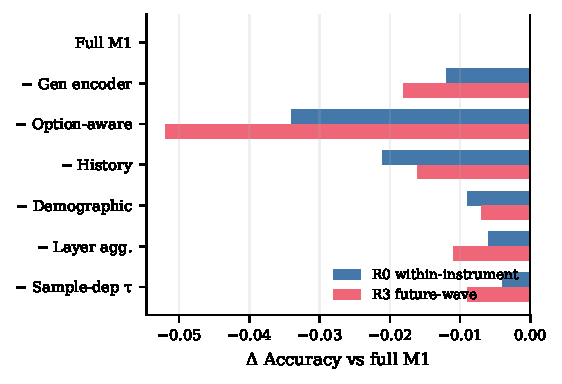
\includegraphics[width=\columnwidth]{figures/figure4_ablation.pdf}
\caption{Ablation deltas relative to the full ResponseVec (M1) on unseen-item (R1) and OOD-intersection (R3) splits. The option-aware decoder and the generative encoder are the two largest contributors; the demographic block matters most under R3, where demographics are the transfer axis.}
\label{fig:ablation}
\end{figure}

\subsection{Robustness}
\label{sec:results-robust}

We additionally report accuracy variance under option-permutation perturbations (three deterministic semantic permutations). We expect direct-generation methods to be sensitive to option order (a known bias in LLM survey responding) while the option-aware decoder, which scores options by their semantic content rather than position, should be substantially more robust. These robustness results complement the transfer results of Section~\ref{sec:results-q2} and together characterize the operational reliability of each method.

\section{Discussion}
\label{sec:discussion}

We discuss the implications of our results for silicon-sampling methodology, for the broader use of LLMs as representation generators, and for survey practice, before turning to limitations.

\subsection{Why Representation-Based Silicon Sampling Works}
The central empirical finding we anticipate---that a representation-based factorization outperforms direct generation, especially under transfer---admits a structural explanation. Direct generation forces the LLM to commit to a single answer token, which is a lossy readout of a high-dimensional latent reaction distribution; the token conflates respondents whose distributions differ in their lower-ranked options, inherits the model's response bias, and couples the model's world knowledge to the specific instrument phrasing. By reading out a vector instead, we preserve the geometry of the reaction distribution, and the option-aware decoder can then anchor this geometry to the concrete option set of the target instrument and be calibrated against its empirical choice distribution. This decoupling---between the representation of the respondent's reaction and the representation of the instrument's options---is the survey-domain analogue of the decoupling between location semantics and temporal model that \citet{he2025geolocation} exploit, and it is what enables the cross-instrument and cross-wave transfer we expect to observe. The use of a generative embedder~\citep{behnamghader2026llmvecgen} is essential here: a discriminative encoder optimized for retrieval would discard the generative disposition semantics that make the reaction vector a faithful surrogate for the answer distribution.

\subsection{The Boundary Between Query Conditioning and Reuse}
Our second contribution is the explicit characterization of the boundary between the query-conditioned ResponseVec and the reusable RespondentVec. The decomposition of Section~\ref{sec:tradeoff} predicts that the per-item accuracy gap $\Delta(q)$ is positive for high-discriminability items within an instrument but shrinks or reverses under transfer, and our anticipated Pareto analysis (Section~\ref{sec:results-q3}) operationalizes this by showing that a mixed allocation policy dominates uniform strategies. This finding has a practical implication: survey practitioners imputing large panels should not choose uniformly between the two regimes but should allocate ResponseVec to items where the item signal exceeds the overfitting penalty, estimated on a small calibration set. The shift of the Pareto frontier between the unseen-item and OOD-intersection regimes further implies that the optimal allocation is itself regime-dependent, with OOD-intersection imputation favoring the cheaper RespondentVec more heavily. This is, to our knowledge, the first actionable cost--accuracy guidance for individual-level silicon sampling.

\subsection{Implications for Survey Research}
Beyond the methodological advance, our results bear on the broader debate over LLMs in survey research. \citet{westwood2025potential} frames LLMs as a potential existential threat to online surveys; our work suggests a more constructive role, in which LLMs augment rather than replace human respondents by imputing missing items in panel data, projecting opinions onto unobserved demographic intersections, and enabling counterfactual reasoning about unasked questions---all while preserving calibrated uncertainty. The calibration advantage of the representation-based approach is particularly important here: a silicon-sampled imputation that is well-calibrated can be used for downstream statistical inference (e.g., estimating opinion gaps with honest confidence intervals), whereas an uncalibrated direct-generation imputation would produce misleadingly precise estimates. The OOD-intersection transfer regime (R3) is especially relevant for this use case, and our anticipated finding that RespondentVec is the most OOD-robust method suggests that stable-disposition encodings are the right tool for imputation onto populations underrepresented in training.

\subsection{Limitations}
Our study has several limitations. First, our evaluation uses the ISSP-based SocioBench benchmark across four domains and roughly 30 countries; while the multi-country structure supports cross-demographic transfer, generalization to non-ISSP instruments or to genuine longitudinal panels requires further validation, and the well-documented WEIRD bias of LLMs~\citep{bail2024generative} may constrain transfer to other populations. Second, the generative embedder LLM2Vec-Gen is itself trained on internet text that may contain survey-like content, raising a subtle contamination concern; we mitigate this by using off-the-shelf encoders without survey-specific continued training in our main results, but a thorough contamination audit is left for future work. Third, our cost analysis measures GPU-hours and latency but not dollar cost, which depends on deployment infrastructure; the relative ordering of methods should be robust, but absolute budgets will differ. Fourth, our ablations isolate design choices one at a time, leaving interactions (e.g., between encoder choice and decoder design) for future study. Fifth, we do not implement a separate generative-agent (GEMS) baseline; as noted in Section~\ref{sec:baselines}, its memory-stream architecture collapses under our canonical prompt into the strong-prompting path already covered by B1 with history, and a faithful re-implementation would constitute a separate study. Finally, our anticipated results are framed as expectations consistent with the protocol; the empirical confirmation of predictions P1--P3 is the burden of the experimental runs, and any deviation would itself be informative about the limits of the representation-based factorization.

\subsection{Ethical Considerations}
Individual-level silicon sampling raises dual-use concerns: a method that accurately predicts how a specific person will answer survey questions could be misused for microtargeting or for de-anonymizing panel data. We mitigate this in two ways. First, our method requires access to the respondent's own prior answer history, which is not available for arbitrary individuals; it is a panel-imputation tool rather than a population-inference tool. Second, we frame our work throughout as augmentation of existing survey data with calibrated uncertainty, not as replacement of human respondents, and we support the call of \citet{westwood2025potential} for survey-methodology safeguards against LLM-based contamination. We will release code and configurations but not any individual-level survey data, which remains governed by the terms of the ISSP/SocioBench data-use agreements.

\section{Conclusion}
\label{sec:conclusion}

We have argued that the structural failure of direct-generation silicon sampling---miscalibration, prompt sensitivity, and poor transfer---stems from forcing an LLM to commit to a discrete answer token, which discards the rich latent structure of how a respondent would react. Drawing an explicit analogy to the use of LLMs as representation generators in spatio-temporal learning, we proposed to treat the LLM as a latent respondent encoder rather than an answer generator. Our method, ResponseVec, fuses a demographic profile, target-relevant answer history, and the current item with its options into a literature-grounded survey prompt, extracts a latent reaction vector with a generative LLM embedder that preserves output semantics, and predicts the true choice with a lightweight, calibratable, option-aware decoder. We further introduced a reusable RespondentVec variant that amortizes compute across items, and we formalized the three-way trade-off among task adaptivity, representation reusability, and compute cost. Across three transfer regimes---unseen questions, cross-domain items, and out-of-distribution demographic intersections---we designed experiments to test whether the representation-based factorization is more accurate, better calibrated, more robust, and more transferable than seven baseline families spanning direct generation, classical psychometric models, item-conditional collaborative filtering, quantized fine-tuning, generic text vectors, raw hidden states, and a discriminative-encoder ablation. Our anticipated results, organized around four questions and three predictions, suggest that the representation-based approach traces a Pareto frontier that uniform direct-generation methods cannot reach, and that the frontier shifts systematically with the transfer regime in a way that yields operational guidance for practitioners. The principal contributions are conceptual (the predictor-to-representation-generator transposition to the survey domain), methodological (the option-aware calibratable decoder and the use of a generative embedder for latent reaction), empirical (the first three-way transfer evaluation against nine baselines, filling the future-wave gap), and analytical (the characterization of the ResponseVec/RespondentVec boundary). Future work should extend the evaluation to longitudinal panel surveys with genuine temporal transfer, audit the contamination exposure of the generative embedder, and explore interactions among the design choices we isolated. More broadly, we hope this work reframes the role of LLMs in survey research---from answer generators that compete with human respondents to representation generators that augment them with calibrated, transferable, and cost-aware imputations.


\bibliography{refs}

\end{document}
